\documentclass[english, 12pt]{article}

\usepackage{amsmath}
\usepackage{amssymb}
\usepackage[style=vancouver, sorting=none, doi=true, urldate=iso, seconds=true, backend=bibtex8]{biblatex}
\usepackage{float}
\usepackage{hyperref}
\usepackage{mathtools}
\usepackage{graphicx}
\usepackage{subcaption}
\usepackage{tkz-euclide}

\usetikzlibrary{arrows.meta, decorations.markings}
\abovecaptionskip=3pt
\parindent=0pt
\parskip=8.0pt
\baselineskip=12pt
\oddsidemargin=-0.5cm
\textwidth=17cm
\topmargin=-1.4cm
\textheight=23.0cm

\addbibresource{references.bib}

\title{MTH3022 Project} % TODO: Decide
\author{Candidate numbers : 196722, 100612}
\date{}

\begin{document}

\maketitle
\section{Introduction}
TODO
\section{Semantic Web}
The semantic web is a set of standards defined by the World Wide Web Consortium\cite{w3c_website} with the goal of allowing computers to parse and understand internet data. The primary technologies they developed for this are the Resource Description Framework\cite{w3c_rdf} (RDF) and the Web Ontology Language\cite{w3c_owl} (OWL).

\subsection{RDF}
The Resource Description Framework is designed to standardise links between subjects and objects, and while it was initially designed for metadata, it is now used generally across a wide variety of domains. At its core are RDF graphs, sets of \texttt{(subject, predicate, object)} triples. \texttt{subject}s and \texttt{object}s are called resources (typically either text or IRIs\cite{iri_rfc}) and denote something that exists, while \texttt{predicates} denote properties and are always IRIs. These depict a relationship between the \texttt{subject} and the \texttt{object}, with \texttt{predicate} indicating the type of relationship. This can be depicted as a directed graph, with \texttt{subject}s and \texttt{object}s being vertices, and \texttt{predicate}s being edge labels. For example the RDF graph \{\texttt{(sky, colour, blue), (sky, above, grass), (sky, above, trees), (grass, colour, green), (trees, colour, green)}\} could be depicted as below.
\begin{figure}[H]
\centering
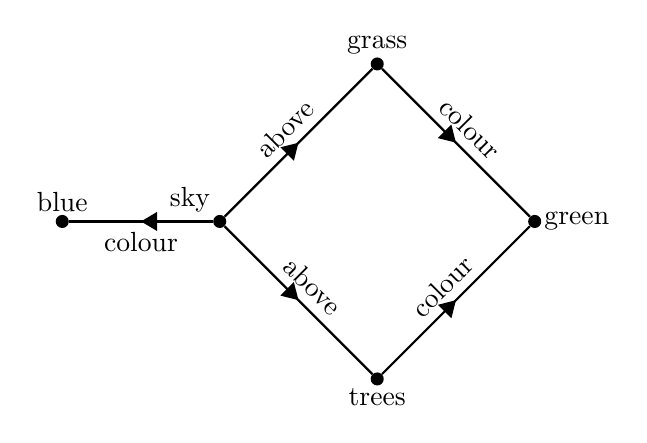
\begin{tikzpicture}
\tkzLabelPoint[above left](0, -2){sky}
\node[circle, fill=black, scale=0.5] at (0, -2) (sky) {};
\tkzLabelPoint[above](2, 0){grass}
\node[circle, fill=black, scale=0.5] at (2, 0) (grass) {};
\tkzLabelPoint[below](2, -4){trees}
\node[circle, fill=black, scale=0.5] at (2, -4) (trees) {};
\tkzLabelPoint[right](4, -2){green}
\node[circle, fill=black, scale=0.5] at (4, -2) (green) {};
\tkzLabelPoint[above](-2, -2){blue}
\node[circle, fill=black, scale=0.5] at (-2, -2) (blue) {};

\begin{scope}[thick,decoration={markings, mark=at position 0.5 with {\arrow{Triangle[scale=1.2]}}}]
\draw[postaction={decorate}] (sky) -- (blue) node[midway, below, sloped]{colour};
\draw[postaction={decorate}] (sky) -- (grass) node[midway, above, sloped]{above};
\draw[postaction={decorate}] (sky) -- (trees) node[midway, above, sloped]{above};
\draw[postaction={decorate}] (grass) -- (green) node[midway, above, sloped]{colour}; 
\draw[postaction={decorate}] (trees) -- (green) node[midway, above, sloped]{colour};
\end{scope}
\end{tikzpicture}
% TODO: Should probably have a caption
\end{figure}

\subsection{OWL}
The Web Ontology Language (OWL) and its successor (OWL2) is designed to be a consistent framework to describe a variety of concepts related the internet. It does this by providing a set of axioms which constrain types of items (called ``classes'') and what relationships are permitted between them. This makes it possible to reason with data created by someone else because they will all use the same terms. OWL generally uses RDF (or a similar format) for describing the actual layout of the data, instead concerning itself with what sort of constraints those relationships model.

There are multiple different types of both OWL and OWL2, designed for different use cases. OWL2 has a general specification \emph{OWL2 DL}\cite{w3c_owl2} and then there exist profiles which remove some of the complexity to make them easier to use for particular domains, while still remaining fully compatible with \emph{DL}. These profiles are \emph{OWL2 EL}, designed for relatively simple reasoning over very large datasets, \emph{OWL2 QL} which allows queries about relationships between items to be answered very efficiently, for example in databases, and \emph{OWL2 RL} which allows the user to reason directly on RDF triples.

\section{Methods}

\subsection*{Notation}

Let $A = (V_A,E_A, \varepsilon_A)$ and $B = (V_B,E_B, \varepsilon_B)$ be two graphs with respective adjacency matrices $\mathbf A_A$ and $\mathbf A_B$.

Let $n_A = |E_A|$, $n_B = |E_B|$ and $m_A = |V_A|$, $m_B = |V_B|$

\subsection{Similarity}
Each vertex has a unique id (a unique name). Two vertices of different graphs {\it match} when they have the same id.
We say that the edges $e_A \in E_A$ and $e_B \in E_B$ are {\it matching} if $\varepsilon_A(e_A)$ and $\varepsilon_B(e_B)$ map to matching vertices.

According to \cite{2019osti}, the {\it similarity} between two networks is the mean of four measurements:
\begin{align*}
\shortintertext{\bf Edge strength similarity $L_S$}
  L_S &= \dfrac{\sum_{i = 1}^n|S_i^A - S_i^B|}{\sum_{i=1}^n|S_i^A + S_i^B|}
\shortintertext{$S_i^A$ and $S_i^B$ are the strength (or weights) of the edge $i$ in both graphs.}
\\
\shortintertext{\bf Matching edge ratio $L_M$}
  L_M &= \dfrac{N_E}{n}
\shortintertext{$N_E$ is the number of edges matching in both networks, and $n$ is the maximum number of edges, $n = \max(n_A,n_B) = \max(|E_A|, |E_B|)$.}
\\
\shortintertext{\bf Vertex ratio $V_M$}
  V_M &= \dfrac{N_V}{m}
\shortintertext{$N_E$ is the number of matching vertices between networks, and $m$ is the total number of vertices, $m = \max(m_A,m_B)=  \max(|V_A|, |V_B|)$.}
\\
\shortintertext{\bf Matching Cluster Ratio $V_C$}
  V_C &= \dfrac{N_C}{m}
\shortintertext{$N_C$ is the number of vertex cluster assignment between networks.}
\end{align*}

According to \cite{2019osti}, the {\bf total similarity} is

$$S = \dfrac{1-L_S + L_M + N_M + N_C}{4},\qquad S \in [0,1]$$

Note that the studied and produced graphs of this paper don't use weighted edges. Thus, to compute the total similarity we don't take into account the {\bf edge strength similarity},
i.e.
$$S = \dfrac{L_M + N_M + N_C}{3},\qquad S \in [0,1]$$

The aim of the total similarity is to see how far it is from one, as two identical graphs will have a total similarity of one.

\subsection{Connectivity and communities}

The {\it vertex connectivity} $\kappa(A)$ of a connected graph $A$ refers to the least cardinality $\kappa(A) = |S|$ of a subset of the vertex set $S \subset V_A$ such that the new graph $\tilde A = (\tilde V_A, \tilde E_A, \tilde \varepsilon_A)$ (with $\tilde V_A = V_A \backslash S$) is either disconnected or trivial.
Such set $S$ is called a {\it minimum vertex cut}.

The {\it strong vertices} are the vertices with a maximum vertex connectivity.
%
\vspace{-.5cm} %otherwise it is a bit "too" far away
%
\paragraph{Computation of the connectivity of a graph:}
Let $N(v_1)$ be the set of all adjacent vertices to $v_1$ (note that if $v_2\in N(v_1)$, then we have $v_1 \in N(v_2)$).\\
Then, for an arbitrary vertex $v_1$:
%
\begin{align*}
\shortintertext{If $\exists S$ s.t. $v_1 \not\in S$, i.e. there is a minimum vertex-cut that does not contain $v_1$ then}
  \kappa(A) &= \min\big\{\kappa(v_1,v_2) \:|\: v_1 \in V_A,\: v_2 \in V_A\backslash\{v_1\},\: \text{and $v_2$ is not adjacent to $v_1$}\big\}\\\\
\shortintertext{If $v_1 \in S,\: \forall S$ then}
  \kappa(A) &= \min\big\{\kappa(v_2,v_3) \:|\: v_2,v_3 \in N(v_1),\:\text{and $v_2,v_1$ are not adjacent}\big\}
\end{align*}

We can compute the connectivity by the maximum flow algorithm proposed by A.H. Esfahanian. \cite[Algorithm 11]{2013Esfahanian}.

% talk about Menger's theorem (?)

The aim of computing the connectivity of a graph is to compare the strong vertices of different graphs. There are two questions to ask:
Do both graphs have the same strong vertex? If they do, how different is their connectivity?\\
If the difference between the connectivity of the strong vertex of each graph is close to zero, both graphs will be considered to have a similar structure.

In this paper we will focus on the communities, they are closely related to the strong vertices since two communities are separated by a strong vertex. They will be computed with the \texttt{Mathematica} function \texttt{FindGraphCommunities}.

\subsection{Spectral distances}

Following \cite{2020Wills}, the $i,j-$th component of an {\it adjacency matrix} is defined as
$$\mathbf A_{i,j} = \begin{cases}1&\text{if}\; i\sim j,\\0&\text{otherwise.}\end{cases}$$
The fact that $A_{i,j} = \{0,1\}$ means that there is at most one edge between two vertices. Thereby we can define the {\it degree} $d_i$ of the vertex $i$ as the number of edges connected to the $i$.

The {\it degree matrix} $\mathbf D$ is a diagonal matrix whose diagonal contains the degree of each vertex.

$$\mathbf D_{i,j} =  \begin{cases}d_i&\text{if}\; i = j,\\0&\text{otherwise.}\end{cases}$$

\paragraph{Spectrum of a matrix}

The {\it spectrum of a matrix} is a sorted sequence of eigenvalues.\\
Let us denote the $i$-th eigenvalue of the adjacency matrix by $\lambda_i^{\mathbf A}$, and the $i$-th eigenvalue of the Laplacian matrix by $\lambda_i^{\mathbf L}$

\paragraph{Adjacency and Laplacian spectral distance}
Let $\lambda^{\mathbf A_A}$ and  $\lambda^{\mathbf A_B}$ be the adjacency spectra of the graphs $A$ and $B$ and let $\lambda^{\mathbf L_A}$ and  $\lambda^{\mathbf L_B}$ be their Laplacian spectra.

Then, the {\bf Adjacency spectral distance} is defined as

$$d_{\mathbf A}(A,B) = \Bigg( \sum_{i=1}^n (\lambda_i^{\mathbf A_A} - \lambda_i^{\mathbf A_B})^2\Bigg)^{1/2}$$

The {\bf Laplacian spectral distance} is defined equivalently, but obviously using the Laplacian spectra.

In this paper, the Adjacency and Laplacian spectral distances will be computed as defined in the \texttt{Week8-ComparingGraphs2023-4} worksheet.

% aim : TODO 
\section{Graph Generation}
To generate our RDF graph we chose to link automatically the maths modules to msc2020\cite{msc_2010} codes. This allowed both a greater degree of objectivity and for us to include all modules on our graph rather than only those we have taken. Notice that each module descriptor has a similar style (except Group Project which we didn't classify as it is too varied). Thereby, we were able to parse their PDF descriptors and only take the ``Syllabus Plan''.

The syllabus plan is then splitted into words which are classified according to the msc2020 code using Mathematica's built-in classifier trained on the entire subject classification (imported as a csv). One of the encoutered problems was the use of pronounds and prepositions (``a'', ``the'', ``as'', ``and'', ``also'', etc) as well as maths ``general'' vocabulary (``mathematics'', ``model'', ``theorem'', etc). As these words were used in several if not all syllabus plans, they shouldn't be classified. To resolve this problem generally (rather than needing to create a list of ignored words) we used the probability that Mathematica assigns to its classifications. For each module we then summed up the probabilities for any shared msc code and ordered them in a decreasing order.

Let us consider first 6 words of MTH1000 (Foundations) as an example :

% To generate our RDF graph linking the maths modules to msc2020\cite{msc_2010} codes we chose to do this automatically from module descriptions rather than manually categorising modules. This allowed both a greater degree of objectivity and for us to include all modules on our graph rather than only those modules we have taken. Each module has a similar style to their module descriptions (except Group Project which we don't classify as it is too varied), so we parse their PDF descriptors and only take the `Syllabus Plan'.

% {\color{red}
% We split the syllabus plan into words and then classify each word to a msc2020 code, using Mathematica's built-in classifier trained on the entire subject classification (imported as a csv). One problem with this is that there are words like `the', `and' and also more specific things like `mathematics' that show up all over the place and therefore shouldn't really be classified to one particular module. To resolve this generally (rather than needing to create a list of ignored words) we used the probability Mathematica assigns to its classifications. For each module we then summed up the probabilities for any shared msc code and ordered them greatest to smallest. We can use the first 6 words of MTH1000 (Foundations) as an example:
% }
\begin{itemize}
\item[1.] We have the following list : 
\{\texttt{Functions, logarithmic, exponential, trigonometric, hyperbolic, Partial}\}
\item[2.] Then we use \texttt{Classifier} to convert the initial list into a list of tuples containing the msc2020 code assigned to the word and its probability : 
\{\texttt{\{26Axx, 0.423802\}, \{11Axx, 0.760049\}, \{34Axx, 0.282966\}, \{42Axx, 0.968698\}, \{35Axx, 0.994287\}, \{35Axx, 0.342177\}}\}
\item[3.] If the tuples have the same msc code (first entry) they are groped togeter and their probability (second entry) is summed up. In this case only the \texttt{35Axx} elements are combined, resulting in the list : \{\texttt{\{35Axx, 1.336464\}, \{42Axx, 0.968698\}, \{11Axx, 0.760049\}, \{26Axx, 0.423802\}, \{34Axx, 0.282966\}}\}
	\item[4.] We normalise these values so that they sum to $1$, ensuring consistency across module descriptors of different length : \{\texttt{\{35Axx, 0.354314\}, \{42Axx, 0.256814\}, \{11Axx, 0.201499\}, \{26Axx, 0.112355\}, \{34Axx, 0.0750179\}}\}
   	\item[5.] Finally, we connect the module code to the msc code if its probability is greater than $0.05$. In this example, all words are connected, but in general this averages out to about $5$ connections per module, although it varies between $2$ and $8$. 
\end{itemize}

\subsection*{Loading other graphs}

In order to compare our graph to the ones generated manually, we import and merge all 5 of the public graphs shared to the forum (thanks to Ben White, Holly Barber, Lucie Johnson, Luke Garner and Donovan Tran). While these all do roughly follow our shared ontology (notably the relationship we want is always marked as \texttt{ex[uses]}), they use different urls to refer to MSC codes so can't directly be combined. Most of these graphs also link to the find grained codes like \texttt{03D65} however there wasn't enough text in these to classify so we instead only link to the more general \texttt{03Axx} codes. Therefore to combine these graphs we first filter them to remove all non-\texttt{ex[used]} relations and use regex to convert all msc codes to a shared format.

The advantage of combining these graphs rather than comparing against any single one of them is that each graph only contains those modules the author has taken and so by combining them we get a more well-rounded view of the modules as a whole. Despite this there are still some modules none of these graphs classify, such as \texttt{MTH1000} and so we removed these nodes from our graph for most comparisons.

\section{Comparation}
Let {\bf RDF ours} denote our graph and {\bf RDF other} denote the graph generated by loading the public graphs shared in the forum. We compute their respective communities using mathematica's built in function \texttt{FindGraphCommunities} and obtain the following graphs :

\begin{figure}[h!]
    \centering
    \begin{subfigure}[b]{0.45\textwidth}
        \centering
        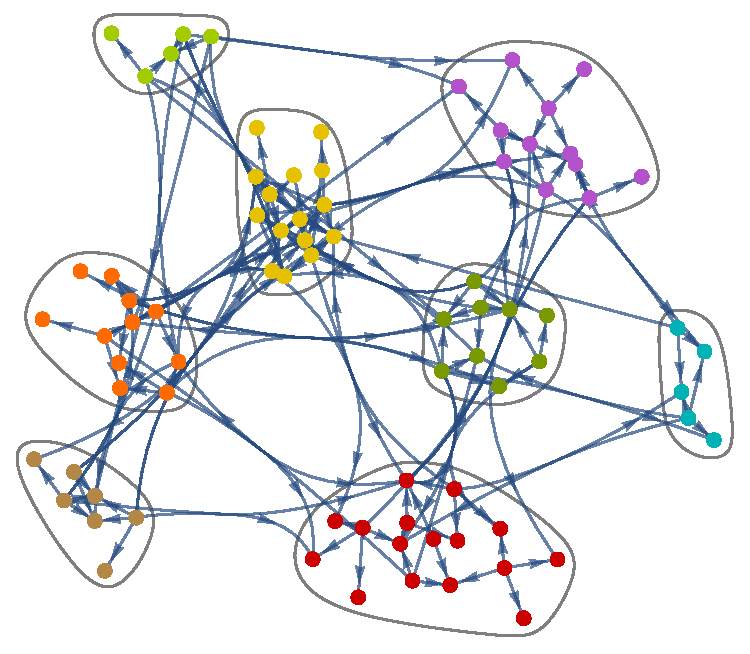
\includegraphics[height=\textwidth]{CommunitiesRDFours.pdf}
        \caption{RDF ours}
    \end{subfigure}%
    ~ 
    \begin{subfigure}[b]{0.45\textwidth}
        \centering
        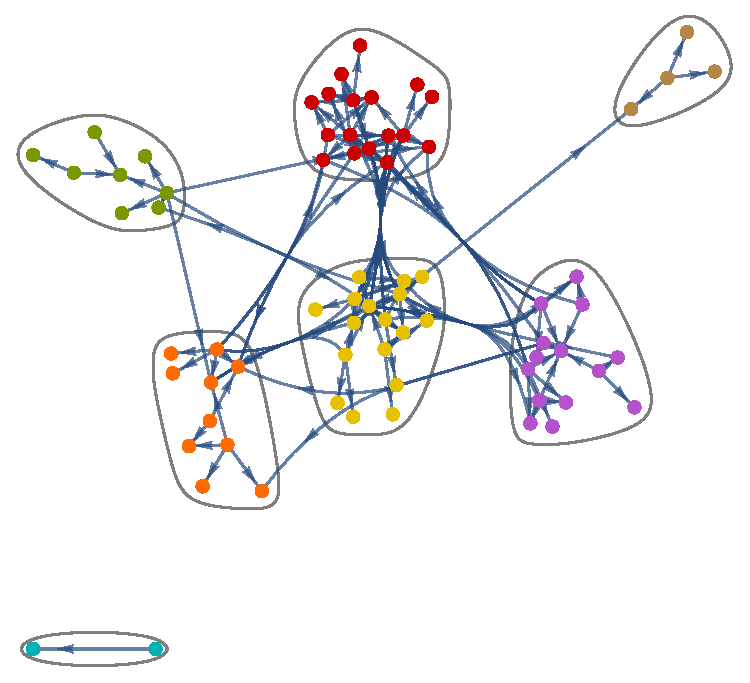
\includegraphics[height=\textwidth]{CommunitiesRDFother.pdf}
        \caption{RDF other}
    \end{subfigure}
    \caption{Communities}
\end{figure}

In {\bf RDF other} graph we find the following communities :

Red : MTH1004, MTH2006, MTH3022, MTH3024, MTH3028 (03-Mathematical logic and foundations, 05-Combinatorics, 15-Linear and multilinear algebra, 41-Approximations and expantions, 60-Probability theory and stochastic processes, 62-Statistics, 68-Computer science, 82-structure of matter, 97-Mathematics education)\\
Yellow : MTH1002, MTH2003, MTH2008, MTH3030, MTH2009, MTH3040 (26-Real functions, 30- 	Functions of a complex variable, 32-Several complex variables and analytic spaces, 33-Special functions, 34-ODEs, 40-Sequences, series, summability, 42-Harmonic analysis on Euclidean spaces, 51-Geometry, 54-General topology, 86-Geophysics, 91-Game theory, economics, finance, and other social and behavioral sciences).\\
Purple : MTH1001, MTH2010, MTH2011, MTH3004, MTH3026, MTH3038, (06-ordered algebraic structures, 08-General algebraic systems, 11-Number theory, 12-Field theory and polynomials, 13-Commutative algebra, 14-Algebraic geometry , 20-Group theory and generalizations, 94-Information and communication theory, circuits)\\
Orange : MTH1003, MTH3006, MTH2005, (00-General and overarching topics; collections, 35-PDEs, 37-Dynamical systems and ergodic theory, 46-Functional analysis, 65-Numerical analysis, 83-Relativity and gravitational theory, 92-Biology and other natural sciences).\\
Green : MTH2004, MTH3007, MTH3001, (53-Differential geometry, 74-Mechanics of deformable solids, 76-Fluid mechanics, 78-Optics, electromagnetic theory, 80-Classical thermodynamics, heat transfer).\\
Brown : MTH3042, (44-Integral transforms, operational calculus, 45-Integral equations, 47-Operator theory).\\
Cyan : MTH3019, (01-History and biography).


In {\bf RDF ours} graph we find the following communities :

Red : MTH1001, MTH2008, MTH2009, MTH3006, MTH3022, MTH3040,  03-Mathematical logic and foundations (05-Combinatorics, 26-Real functions, 28-Real functions, 32-Several complex variables and analytic spaces, 40-Sequences, series, summability, 46-Functional analysis, 54-General topology, 70-Mechanics of particles and systems, 94-Information and communication theory, circuits).\\
Yellow : MTH1000, MTH2003, MTH2005, MTH3004, MTH3026, MTH3039, 65-Numerical analysis, 97-Mathematics education (11-Number Theory, 42-Harmonic analysis on Euclidean spaces, 34-ODEs, 35-PDEs, 68-Computer science, 16-Associative rings and algebras, 55-Algebraic topology)\\
Purple : MTH1003, MTH2004, MTH3001, MTH3007 (31-Potential theory, 00-General and overarching topics; collections, 83-Relativity and gravitational theory, 39-Difference and functional equations, 76-Fluid mechanics, 91-Game theory, economics, finance, and other social and behavioral sciences, 80-Classical thermodynamics, heat transfe, 01-History and biography).\\
Orange : MTH2006, MTH3030, MTH3011, MTH3045 (41-Approximations and expansions, 30-Functions of a complex variable, 81-Quantum theory, 82-Statistical mechanics, structure of matter, 93-Systems theory; control {For optimal control, 49-Calculus of variations and optimal control; optimization, 74-Mechanics of deformable solids).\\
Dark Green : MTH1002, MTH2011, MTH3008, MTH3042 (45-Integral equations, 15-Linear and multilinear algebra; matrix theory, 44-Integral transforms, operational calculus, 47-Operator theory, 37-Dynamical systems and ergodic theory).\\
Gold : MTH1004, MTH3024, MTH3041 (60-Probability theory and stochastic processes, 62-Statistics, 52-Convex and discrete geometry, 18-Category theory; homological algebra)\\
Teal : MTH2010, MTH3038 (20-Group theory and generalizations, 13-Commutative algebra, 12-Field theory and polynomials).\\
Light green : MTH3013, MTH3019, MTH3028 (51-Geometry, 86-Geophysics).


\section{Conclusion}
TODO
\newpage
\printbibliography

  
\end{document}
